\documentclass[a4paper,11pt]{article}
\usepackage[utf8]{inputenc}
\usepackage[T1]{fontenc}
\usepackage{amsmath,amssymb}
\usepackage[a4paper,left=2cm,right=2cm,top=3.6cm,bottom=2.3cm,headheight=1.1cm,headsep=0.6cm,footskip=1cm]{geometry}
\usepackage{xcolor}
\usepackage{tikz}
\usetikzlibrary{calc,arrows.meta,positioning,shapes.geometric}
\usepackage{fancyhdr}
\usepackage{lastpage}
\usepackage{tabularx}
\usepackage{array}
\usepackage[most]{tcolorbox}
\usepackage{enumitem}
\usepackage{needspace}

\definecolor{mainc}{HTML}{075985}
\definecolor{accc}{HTML}{0284C7}
\definecolor{skyl}{HTML}{BAE6FD}
\definecolor{deepc}{HTML}{082F49}
\definecolor{softbg}{HTML}{F0F9FF}
\definecolor{warmc}{HTML}{D97706}
\definecolor{brick}{HTML}{B91C1C}
\newcommand{\dis}{\displaystyle}

\setlength{\parindent}{0pt}
\renewcommand{\arraystretch}{1.35}

\tikzset{
  ar/.style={-{Stealth[length=1.8mm]},thick,mainc},
  box/.style={draw=mainc,thick,rounded corners=3pt,fill=softbg,align=center,inner sep=4pt}
}
\newcommand{\axs}[4]{\draw[->,thick,mainc] (#1,0)--(#3,0) node[right,font=\scriptsize]{$x$};
  \draw[->,thick,mainc] (0,#2)--(0,#4) node[above,font=\scriptsize]{$y$};}

\pagestyle{fancy}
\fancyhf{}
\renewcommand{\headrulewidth}{0pt}
\fancyhead[L]{%
  \begin{tikzpicture}[remember picture,overlay]
    \fill[mainc] ([yshift=-1.2cm]current page.north west) rectangle ([yshift=-3.15cm]current page.north east);
    \fill[skyl] ([yshift=-3.15cm]current page.north west) rectangle ([yshift=-3.3cm]current page.north east);
  \end{tikzpicture}%
  \color{white}\bfseries\large Latihan Soal Integral}
\fancyhead[R]{\color{white}\small Diunduh dari website \textbf{Math1729}\ \,|\,\ 5 Oktober 2026}
\fancyfoot[L]{\small\color{mainc}Math1729 --- Integral}
\fancyfoot[R]{\small\color{mainc}Halaman \thepage\ dari \pageref{LastPage}}

\newcounter{no}
\newcommand{\bagian}[2]{\par\Needspace{6\baselineskip}\vspace{1.0em}\noindent
  \begin{tcolorbox}[colback=mainc,colframe=mainc,coltext=white,boxrule=0pt,arc=2pt,left=6pt,right=6pt,top=3pt,bottom=3pt]
  \textbf{#1}\hfill{\small #2}\end{tcolorbox}\setcounter{no}{0}\par\vspace{-0.3em}}
\newcommand{\tingkat}[2]{\par\Needspace{7\baselineskip}\vspace{0.6em}\noindent
  {\color{accc}\rule{3pt}{1.1em}}\ {\color{mainc}\bfseries #1}\ {\small\color{gray}--- #2}\par\vspace{0.1em}}
\newcommand{\soal}[2]{\par\vspace{0.75em}\stepcounter{no}\noindent
  \begin{minipage}[t]{1.8em}\textbf{\theno.}\end{minipage}%
  \begin{minipage}[t]{\dimexpr\linewidth-1.8em\relax}#1\par\vspace{0.35em}#2\end{minipage}\par}
\newcommand{\poin}[1]{\hfill{\small\color{mainc}[#1 poin]}}
\newcommand{\gbr}[2]{\noindent\begin{minipage}[t]{0.56\linewidth}#1\end{minipage}\hfill\raisebox{\ht\strutbox}{\begin{minipage}[t]{0.41\linewidth}\vspace{0pt}\centering#2\end{minipage}}}
\newcommand{\pil}[5]{\begin{tabularx}{\linewidth}{@{}*{5}{X}@{}}\textbf{A.}\;#1 & \textbf{B.}\;#2 & \textbf{C.}\;#3 & \textbf{D.}\;#4 & \textbf{E.}\;#5\end{tabularx}}
\newcommand{\pilx}[5]{\begin{tabularx}{\linewidth}{@{}*{3}{X}@{}}\textbf{A.}\;#1 & \textbf{B.}\;#2 & \textbf{C.}\;#3\\[10pt] \textbf{D.}\;#4 & \textbf{E.}\;#5 & \end{tabularx}}
\newcommand{\pill}[5]{\begin{tabularx}{\linewidth}{@{}lX@{}}\textbf{A.} & #1\\ \textbf{B.} & #2\\ \textbf{C.} & #3\\ \textbf{D.} & #4\\ \textbf{E.} & #5\end{tabularx}}
\newcommand{\jwb}{\hfill Jawaban: \rule{4.5cm}{0.4pt}}
\begin{document}
\thispagestyle{fancy}

\begin{center}
  {\color{mainc}\fontsize{22}{26}\selectfont\bfseries Latihan Soal Integral\par}
  \vspace{2pt}
  {\color{accc}\large Antiturunan, Teknik Integrasi, Integral Tentu, Luas, Volume Benda Putar, dan Penalaran Kalkulus\par}
\end{center}
\vspace{2pt}
\begin{tcolorbox}[colback=softbg,colframe=mainc!40,boxrule=0.6pt,arc=3pt,left=8pt,right=8pt,top=5pt,bottom=5pt]
\noindent\textbf{Nama} : \rule{4.6cm}{0.4pt}\hfill\textbf{Kelas} : \rule{2.2cm}{0.4pt}\hfill\textbf{Skor} : \rule{2.2cm}{0.4pt}
\end{tcolorbox}
\vspace{2pt}
\begin{tcolorbox}[colback=white,colframe=accc,boxrule=0.8pt,arc=3pt,left=8pt,right=8pt,top=4pt,bottom=4pt,title={\bfseries Petunjuk Pengerjaan},coltitle=white,fonttitle=\small]
\small
\begin{enumerate}[leftmargin=1.4em,itemsep=1pt,topsep=1pt]
\item Soal terdiri atas \textbf{20 pilihan ganda} (5 mudah, 6 sedang, 7 sulit, 2 HOTS), \textbf{5 isian singkat} (2 sedang, 3 sulit), dan \textbf{5 uraian (essay)} (2 sedang, 2 sulit, 1 HOTS). Soal disusun berjenjang dan memakai bentuk yang sejalan dengan UTBK-SNBT dan TKA Matematika 2026: pilihan ganda lima opsi, pilihan ganda kompleks \emph{kategori} (benar/salah tiap pernyataan), pilihan ganda kompleks \emph{MCMA} (pilih semua pernyataan yang benar), kecukupan data, soal berbasis grafik atau gambar, soal berkonteks, dan isian singkat. Alokasi waktu yang disarankan: 120 menit.
\item Skor: pilihan ganda 2 poin, isian singkat 4 poin, uraian 8 poin per soal (total 100 poin). Tidak ada pengurangan skor untuk jawaban salah.
\item Pada soal pilihan ganda kompleks, periksa \textbf{setiap} pernyataan sebelum memilih opsi. Pada soal berbasis gambar, gambar tidak selalu digambar sesuai skala; andalkan angka dan keterangan yang tertera.
\item Bilangan ribuan ditulis dengan tanda titik dan bilangan desimal dengan tanda koma. Pada isian singkat, tuliskan hanya jawaban akhir dalam bentuk eksak (pecahan, $\pi$, atau $e$ boleh dibiarkan).
\item Kalkulator tidak diperkenankan. Konstanta $C$ tidak perlu ditulis pada integral tentu. $\ln$ menyatakan logaritma natural.
\end{enumerate}
\end{tcolorbox}

% =====================================================================
\bagian{A. Pilihan Ganda}{20 soal $\times$ 2 poin = 40 poin. Pilih satu jawaban yang paling tepat.}

\tingkat{Tingkat Mudah}{soal 1 sampai 5}
\soal{Fungsi $F(x)=x^3-2x^2-2$ adalah salah satu antiturunan dari fungsi $f$. Nilai $\dis\int_1^3 f(x)\,dx$ adalah \dots.}{\pil{$-10$}{$-3$}{$4$}{$7$}{$10$}}
\soal{Nilai dari $\dis\int_1^4\left(\dfrac{6}{\sqrt x}+1\right)dx$ adalah \dots.}{\pil{$3$}{$6$}{$9$}{$12$}{$15$}}
\soal{Hasil dari $\dis\int\left(e^{2x}+\cos4x\right)dx$ adalah \dots.}{\pilx{$e^{2x}+\sin4x+C$}{$\dfrac12e^{2x}+\dfrac14\sin4x+C$}{$\dfrac12e^{2x}-\dfrac14\sin4x+C$}{$2e^{2x}-4\sin4x+C$}{$\dfrac12e^{2x}+4\sin4x+C$}}
\soal{\gbr{Gambar menunjukkan grafik fungsi $f$ pada selang $[0,7]$. Tiga daerah yang dibatasi grafik dan sumbu $x$ memiliki luas $6$, $4$, dan $5$ satuan luas seperti tertera pada gambar. Nilai $\dis\int_0^7 f(x)\,dx$ adalah \dots.}{%
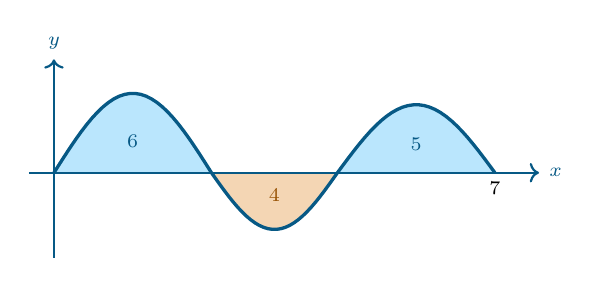
\begin{tikzpicture}[x=0.8cm,y=0.72cm]
\fill[skyl] (0,0) -- plot[domain=0:2.5,samples=30] ({\x},{1.4*sin(180*\x/2.5)}) -- cycle;
\fill[warmc!30] (2.5,0) -- plot[domain=2.5:4.5,samples=30] ({\x},{-1.0*sin(180*(\x-2.5)/2)}) -- cycle;
\fill[skyl] (4.5,0) -- plot[domain=4.5:7,samples=30] ({\x},{1.2*sin(180*(\x-4.5)/2.5)}) -- cycle;
\draw[very thick,mainc,samples=30] plot[domain=0:2.5] ({\x},{1.4*sin(180*\x/2.5)}) plot[domain=2.5:4.5] ({\x},{-1.0*sin(180*(\x-2.5)/2)}) plot[domain=4.5:7] ({\x},{1.2*sin(180*(\x-4.5)/2.5)});
\axs{-0.4}{-1.5}{7.7}{2.0}
\node[font=\scriptsize\bfseries,mainc] at (1.25,0.55) {$6$};
\node[font=\scriptsize\bfseries,warmc!70!black] at (3.5,-0.4) {$4$};
\node[font=\scriptsize\bfseries,mainc] at (5.75,0.5) {$5$};
\node[font=\scriptsize,below] at (7,0) {$7$};
\end{tikzpicture}}}{\pil{$-3$}{$2$}{$5$}{$7$}{$15$}}
\soal{Tentukan nilai kebenaran tiga pernyataan berikut (B = benar, S = salah), berurutan dari (i) sampai (iii).\par\smallskip
(i) $\dis\int_{-1}^{1}\left(x^2+x^3\right)dx=\dfrac23$.\par
(ii) $\dis\int\dfrac1x\,dx=\ln x+C$ berlaku untuk setiap $x\neq0$.\par
(iii) $\dis\dfrac{d}{dx}\int_1^{x}\sqrt{t^3+1}\,dt=\sqrt{x^3+1}$ untuk $x>1$.}{\pilx{B, S, B}{B, B, B}{S, B, B}{B, B, S}{S, S, B}}

\tingkat{Tingkat Sedang}{soal 6 sampai 11}
\soal{Nilai dari $\dis\int_1^{e}\dfrac{(\ln x)^2}{x}\,dx$ adalah \dots.}{\pil{$\frac13$}{$\frac12$}{$\frac23$}{$1$}{$\frac{e^3-1}{3}$}}
\soal{Nilai dari $\dis\int_1^{e}x^2\ln x\,dx$ adalah \dots.}{\pilx{$\dfrac13$}{$\dfrac{e^3+1}{9}$}{$\dfrac{2e^3+1}{9}$}{$\dfrac{2e^3-1}{9}$}{$\dfrac{4e^3-1}{9}$}}
\soal{\gbr{Gambar menunjukkan grafik $y=x^3-4x$. Luas \textbf{seluruh} daerah yang dibatasi kurva tersebut dan sumbu $x$ (daerah berwarna) adalah \dots\ satuan luas.}{%
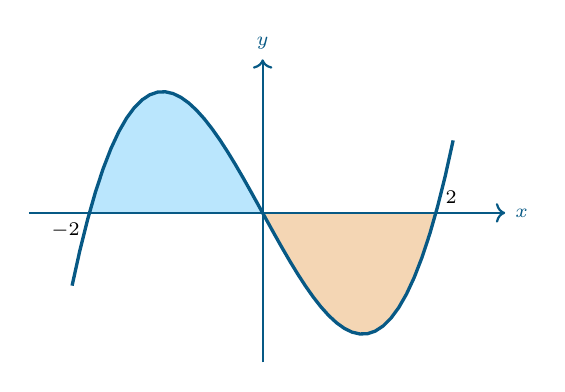
\begin{tikzpicture}[x=1.1cm,y=0.5cm]
\fill[skyl] (-2,0) -- plot[domain=-2:0,samples=30] ({\x},{\x*\x*\x-4*\x}) -- cycle;
\fill[warmc!30] (0,0) -- plot[domain=0:2,samples=30] ({\x},{\x*\x*\x-4*\x}) -- cycle;
\draw[very thick,mainc,domain=-2.2:2.2,samples=50] plot ({\x},{\x*\x*\x-4*\x});
\axs{-2.7}{-3.8}{2.8}{3.9}
\node[font=\scriptsize,below left] at (-2,0) {$-2$};
\node[font=\scriptsize,above right] at (2,0) {$2$};
\end{tikzpicture}}}{\pil{$0$}{$4$}{$8$}{$12$}{$16$}}
\soal{\gbr{Daerah di bawah kurva $y=\sin x$ untuk $0\le x\le\pi$ (berwarna) diputar $360^\circ$ mengelilingi sumbu $x$ sehingga terbentuk benda seperti pada gambar. Volume benda putar tersebut adalah \dots\ satuan volume.}{%
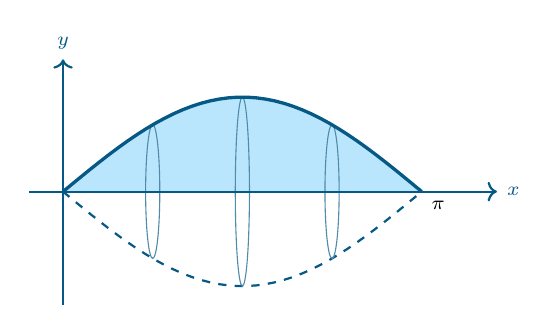
\begin{tikzpicture}[x=1.45cm,y=1.2cm]
\fill[skyl] (0,0) -- plot[domain=0:3.14159,samples=40] ({\x},{sin(\x r)}) -- cycle;
\draw[mainc,dashed,thick,domain=0:3.14159,samples=40] plot ({\x},{-sin(\x r)});
\foreach \c in {0.7854,1.5708,2.3562}{\draw[mainc!70] (\c,0) ellipse ({0.09cm} and {1.2cm*sin(\c r)});}
\draw[very thick,mainc,domain=0:3.14159,samples=40] plot ({\x},{sin(\x r)});
\draw[->,thick,mainc] (-0.3,0)--(3.8,0) node[right,font=\scriptsize]{$x$};
\draw[->,thick,mainc] (0,-1.2)--(0,1.4) node[above,font=\scriptsize]{$y$};
\node[font=\scriptsize,below right] at (3.14159,0) {$\pi$};
\end{tikzpicture}}}{\pil{$2\pi$}{$\pi^2$}{$\frac{\pi^2}{4}$}{$\frac{\pi^2}{2}$}{$\pi$}}
\soal{Sebuah drone mainan bergerak pada lintasan lurus dengan percepatan $a(t)=6-2t$ m/s$^2$ ($t$ dalam detik). Pada saat $t=0$ drone berada di titik asal dan sedang bergerak mundur dengan kecepatan $5$ m/s. Jarak total yang ditempuh drone selama $0\le t\le5$ adalah \dots\ m.}{\pil{$\frac{25}{3}$}{$\frac{32}{3}$}{$11$}{$13$}{$\frac{41}{3}$}}
\soal{Kurva $y=f(x)$ memenuhi $f''(x)=6x-4$, melalui titik $(0,3)$, dan memiliki titik stasioner di $x=1$. Nilai $f(2)$ adalah \dots.}{\pil{$3$}{$5$}{$7$}{$9$}{$11$}}

\tingkat{Tingkat Sulit}{soal 12 sampai 18, setara UTBK}
\soal{Nilai dari $\dis\int_0^{\pi/2}\sin^3x\cos^2x\,dx$ adalah \dots.}{\pil{$\frac1{15}$}{$\frac2{15}$}{$\frac15$}{$\frac4{15}$}{$\frac13$}}
\soal{\gbr{Gambar menunjukkan kurva $y=x^2$ dan $y=\dfrac8x$ yang berpotongan di titik $(2,4)$. Luas daerah yang dibatasi kedua kurva dan garis $x=1$ (daerah berwarna) adalah \dots\ satuan luas.}{%
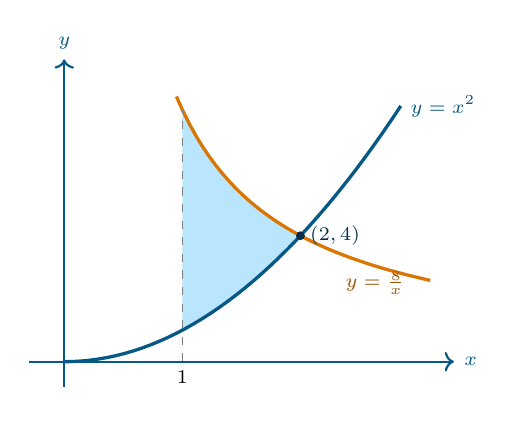
\begin{tikzpicture}[x=1.5cm,y=0.4cm]
\fill[skyl] (1,1) -- (1,8) -- plot[domain=1:2,samples=30] ({\x},{8/\x}) -- plot[domain=2:1,samples=30] ({\x},{\x*\x}) -- cycle;
\draw[very thick,mainc,domain=0:2.85,samples=40] plot ({\x},{\x*\x});
\draw[very thick,warmc,domain=0.95:3.1,samples=40] plot ({\x},{8/\x});
\draw[dashed,gray] (1,0)--(1,8);
\axs{-0.3}{-0.8}{3.3}{9.6}
\fill[deepc] (2,4) circle (1.6pt) node[right,font=\scriptsize]{$(2,4)$};
\node[font=\scriptsize,below] at (1,0) {$1$};
\node[font=\scriptsize,mainc,right] at (2.85,8.1) {$y=x^2$};
\node[font=\scriptsize,warmc!70!black,right] at (2.3,2.5) {$y=\frac8x$};
\end{tikzpicture}}}{\pilx{$\dfrac73-8\ln2$}{$4\ln2-\dfrac73$}{$8\ln2-\dfrac83$}{$8\ln2-\dfrac73$}{$8\ln2+\dfrac73$}}
\soal{Nilai dari $\dis\int_0^3\dfrac{x}{\sqrt{x+1}}\,dx$ adalah \dots.}{\pil{$\frac23$}{$\frac43$}{$\frac83$}{$\frac{10}3$}{$\frac{16}3$}}
\soal{Fungsi $f$ kontinu pada $[0,6]$ dengan $\dis\int_1^5 f(x)\,dx=12$. Pilih \textbf{semua} pernyataan yang benar.\par\smallskip
(1) $\dis\int_0^2 x\,f(x^2+1)\,dx=6$.\par
(2) $\dis\int_0^2 f(2x+1)\,dx=12$.\par
(3) $\dis\int_1^5\big[f(x)+2\big]\,dx=20$.\par
(4) $\dis\int_1^5 f(6-x)\,dx=-12$.}{\pill{(1), (2), dan (3) saja}{(2) dan (4) saja}{(1), (3), dan (4) saja}{(1) dan (4) saja}{(1) dan (3) saja}}
\soal{Nilai dari $\dis\int_0^{\pi}e^x\sin x\,dx$ adalah \dots.}{\pilx{$\dfrac{e^\pi-1}{2}$}{$\dfrac{e^\pi}{2}$}{$\dfrac{e^\pi+1}{2}$}{$e^\pi-1$}{$e^\pi+1$}}
\soal{\gbr{Daerah yang dibatasi parabola $y=x^2$ dan $y=2-x^2$ (berwarna) diputar $360^\circ$ mengelilingi sumbu $x$. Volume benda putar yang terbentuk adalah \dots\ satuan volume.}{%
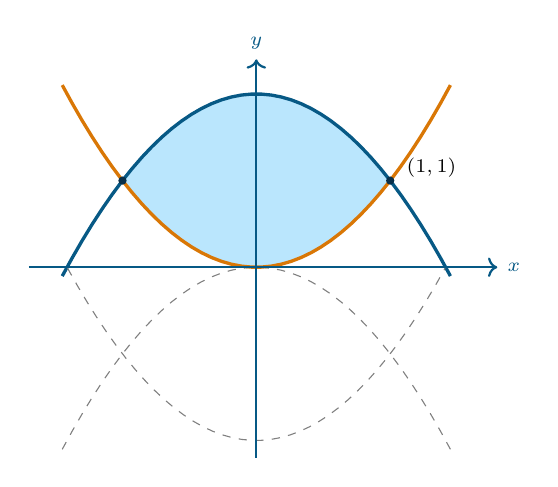
\begin{tikzpicture}[x=1.7cm,y=1.1cm]
\fill[skyl] plot[domain=-1:1,samples=30] ({\x},{2-\x*\x}) -- plot[domain=1:-1,samples=30] ({\x},{\x*\x}) -- cycle;
\draw[very thick,mainc,domain=-1.45:1.45,samples=40] plot ({\x},{2-\x*\x});
\draw[very thick,warmc,domain=-1.45:1.45,samples=40] plot ({\x},{\x*\x});
\draw[dashed,gray,domain=-1.45:1.45,samples=40] plot ({\x},{-\x*\x});
\draw[dashed,gray,domain=-1.41:1.41,samples=40] plot ({\x},{-(2-\x*\x)});
\axs{-1.7}{-2.2}{1.8}{2.4}
\fill[deepc] (1,1) circle (1.5pt) (-1,1) circle (1.5pt);
\node[font=\scriptsize,right] at (1.05,1.15) {$(1,1)$};
\end{tikzpicture}}}{\pil{$2\pi$}{$\frac{8\pi}{3}$}{$4\pi$}{$\frac{64\pi}{15}$}{$\frac{16\pi}{3}$}}
\soal{\gbr{Daerah di bawah kurva $y=x^2$ pada selang $[1,3]$ didekati dengan $n$ persegi panjang beralas sama (jumlah Riemann kanan, gambar untuk $n=5$). Nilai $\dis\lim_{n\to\infty}\sum_{k=1}^{n}\dfrac2n\left(1+\dfrac{2k}{n}\right)^2$ adalah \dots.}{%
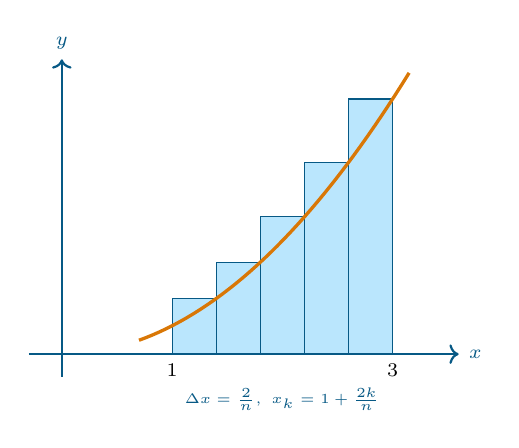
\begin{tikzpicture}[x=1.4cm,y=0.36cm]
\foreach \k in {1,...,5}{\pgfmathsetmacro{\xa}{1+0.4*(\k-1)}\pgfmathsetmacro{\xb}{1+0.4*\k}
 \draw[fill=skyl,draw=mainc] (\xa,0) rectangle (\xb,{\xb*\xb});}
\draw[very thick,warmc,domain=0.7:3.15,samples=40] plot ({\x},{\x*\x});
\axs{-0.3}{-0.8}{3.6}{10.4}
\node[font=\scriptsize,below] at (1,0) {$1$};
\node[font=\scriptsize,below] at (3,0) {$3$};
\node[font=\tiny,mainc] at (2,-1.6) {$\Delta x=\frac2n,\ x_k=1+\frac{2k}{n}$};
\end{tikzpicture}}}{\pil{$\frac83$}{$\frac{26}{3}$}{$9$}{$\frac{28}{3}$}{$12$}}

\tingkat{Tingkat HOTS}{soal 19 dan 20, penalaran tingkat tinggi gaya UTBK}
\soal{Diketahui $f(x)=ax^2+bx$ dengan $a$ dan $b$ konstanta. Berapakah nilai $\dis\int_0^3 f(x)\,dx$?
\begin{enumerate}[label=(\arabic*),leftmargin=1.8em,itemsep=0pt,topsep=2pt]
\item Grafik $f$ memiliki garis singgung mendatar di titik dengan absis $x=1$.
\item $f(1)=-1$.
\end{enumerate}}{\begin{tabularx}{\linewidth}{@{}lX@{}}
\textbf{A.} & Pernyataan (1) SAJA cukup untuk menjawab pertanyaan, tetapi pernyataan (2) SAJA tidak cukup.\\
\textbf{B.} & Pernyataan (2) SAJA cukup untuk menjawab pertanyaan, tetapi pernyataan (1) SAJA tidak cukup.\\
\textbf{C.} & DUA pernyataan BERSAMA-SAMA cukup untuk menjawab pertanyaan, tetapi SATU pernyataan SAJA tidak cukup.\\
\textbf{D.} & Pernyataan (1) SAJA cukup dan pernyataan (2) SAJA cukup untuk menjawab pertanyaan.\\
\textbf{E.} & Pernyataan (1) dan pernyataan (2) tidak cukup untuk menjawab pertanyaan.
\end{tabularx}}
\soal{\gbr{Grafik $f$ pada selang $[0,8]$ tersusun dari ruas-ruas garis lurus yang menghubungkan titik $(0,0)$, $(1,2)$, $(3,2)$, $(5,-2)$, $(6,-2)$, dan $(8,2)$. Misalkan $F(x)=\dis\int_0^x f(t)\,dt$ untuk $0\le x\le8$. Pilih \textbf{semua} pernyataan yang benar.\par\smallskip
(1) $F$ mencapai nilai terbesarnya pada $x=4$.\par
(2) $F(6)=3$.\par
(3) $F$ turun pada selang $3<x<7$.\par
(4) $\dis\int_0^8 f(x)\,dx=11$.}{%
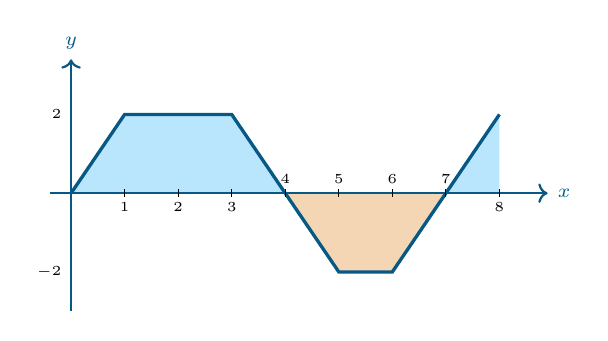
\begin{tikzpicture}[x=0.68cm,y=0.5cm]
\fill[skyl] (0,0)--(1,2)--(3,2)--(4,0)--cycle;
\fill[warmc!30] (4,0)--(5,-2)--(6,-2)--(7,0)--cycle;
\fill[skyl] (7,0)--(8,2)--(8,0)--cycle;
\draw[very thick,mainc] (0,0)--(1,2)--(3,2)--(5,-2)--(6,-2)--(8,2);
\axs{-0.4}{-3}{8.9}{3.4}
\foreach \t/\pos in {1/below,2/below,3/below,4/above,5/above,6/above,7/above,8/below}{\draw (\t,0.1)--(\t,-0.1); \node[font=\tiny,\pos] at (\t,0) {\t};}
\node[font=\tiny,left] at (0,2) {$2$}; \node[font=\tiny,left] at (0,-2) {$-2$};
\end{tikzpicture}}}{\pill{(1) dan (2) saja}{(1), (2), dan (4) saja}{(2) dan (3) saja}{(3) dan (4) saja}{(1) dan (3) saja}}

% =====================================================================
\bagian{B. Isian Singkat}{5 soal $\times$ 4 poin = 20 poin. Tuliskan hanya jawaban akhir.}

\tingkat{Tingkat Sedang}{soal 1 dan 2}
\soal{Diketahui $\dis\int_1^{a}(4x-3)\,dx=6$ dengan $a>1$. Nilai $a$ adalah \dots.}{\jwb}
\soal{\gbr{Air mengalir ke dalam sebuah bak dengan laju $r(t)$ liter/menit, $0\le t\le10$, seperti pada grafik (tersusun dari ruas garis lurus). Pada saat $t=0$ bak sudah berisi $5$ liter air. Banyak air dalam bak pada saat $t=10$ adalah \dots\ liter.}{%
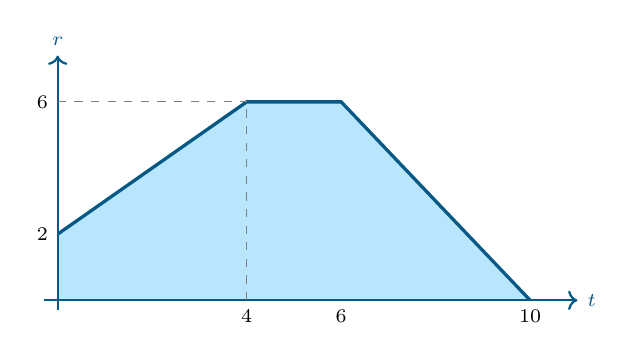
\begin{tikzpicture}[x=0.6cm,y=0.42cm]
\fill[skyl] (0,0)--(0,2)--(4,6)--(6,6)--(10,0)--cycle;
\draw[very thick,mainc] (0,2)--(4,6)--(6,6)--(10,0);
\draw[->,thick,mainc] (-0.3,0)--(11,0) node[right,font=\scriptsize]{$t$};
\draw[->,thick,mainc] (0,-0.3)--(0,7.4) node[above,font=\scriptsize]{$r$};
\foreach \t in {4,6,10}{\node[font=\scriptsize,below] at (\t,0) {$\t$};}
\node[font=\scriptsize,left] at (0,2) {$2$}; \node[font=\scriptsize,left] at (0,6) {$6$};
\draw[dashed,gray] (4,0)--(4,6) (0,6)--(4,6);
\end{tikzpicture}}}{\jwb}

\tingkat{Tingkat Sulit}{soal 3 sampai 5}
\soal{Nilai dari $\dis\int_0^{\pi/6}\sin3x\cos x\,dx$ adalah \dots.}{\jwb}
\soal{Fungsi $f$ kontinu dan memenuhi $f(x)=3x^2+2\dis\int_0^1 f(t)\,dt$ untuk setiap bilangan real $x$. Nilai $f(2)$ adalah \dots.}{\jwb}
\soal{\gbr{Garis $g$ menyinggung parabola $y=x^2$ di titik $(2,4)$. Luas daerah yang dibatasi parabola, garis $g$, dan sumbu $x$ (daerah berwarna) adalah \dots\ satuan luas.}{%
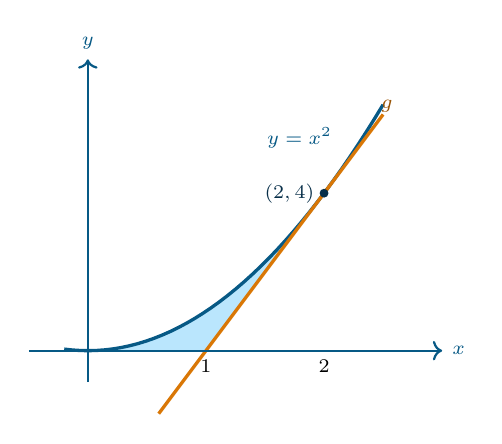
\begin{tikzpicture}[x=1.5cm,y=0.5cm]
\fill[skyl] (0,0)--(1,0)--(2,4)--plot[domain=2:0,samples=30] ({\x},{\x*\x})--cycle;
\draw[very thick,mainc,domain=-0.2:2.5,samples=40] plot ({\x},{\x*\x});
\draw[very thick,warmc,domain=0.6:2.5] plot ({\x},{4*\x-4});
\axs{-0.5}{-0.8}{3.0}{7.4}
\fill[deepc] (2,4) circle (1.6pt) node[left,font=\scriptsize]{$(2,4)$};
\node[font=\scriptsize,below] at (1,0) {$1$}; \node[font=\scriptsize,below] at (2,0) {$2$};
\node[font=\scriptsize,warmc!70!black,right] at (2.4,6.2) {$g$};
\node[font=\scriptsize,mainc,left] at (2.15,5.4) {$y=x^2$};
\end{tikzpicture}}}{\jwb}

% =====================================================================
\Needspace{16\baselineskip}
\bagian{C. Uraian (Essay)}{5 soal $\times$ 8 poin = 40 poin. Tuliskan langkah penyelesaian dengan lengkap.}

\tingkat{Tingkat Sedang}{soal 1 dan 2}
\soal{\gbr{Daerah $D$ dibatasi oleh parabola $y=4x-x^2$ dan garis $y=x$ (lihat gambar).\par\smallskip
(a) Tentukan koordinat titik potong kedua kurva.\par
(b) Hitung luas daerah $D$.\par
(c) Hitung volume benda putar jika $D$ diputar $360^\circ$ mengelilingi sumbu $x$.\par
(d) Garis $x=k$ dengan $0<k<3$ membagi $D$ menjadi dua bagian yang luasnya sama. Tentukan $k$ dan jelaskan alasan kesimetrian yang dipakai.}{%
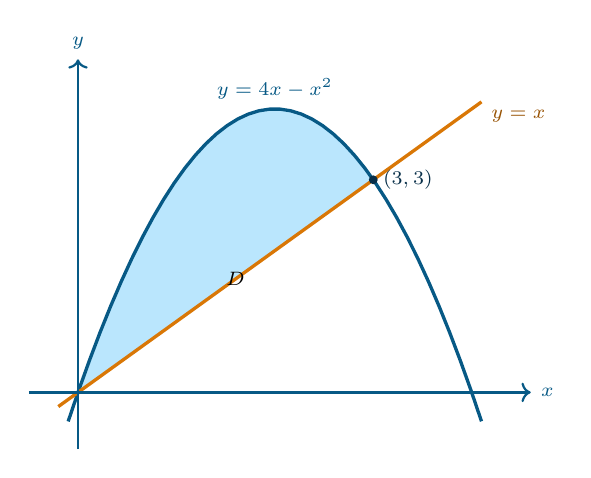
\begin{tikzpicture}[x=1.25cm,y=0.9cm]
\fill[skyl] (0,0)--(3,3)--plot[domain=3:0,samples=30] ({\x},{4*\x-\x*\x})--cycle;
\draw[very thick,mainc,domain=-0.1:4.1,samples=40] plot ({\x},{4*\x-\x*\x});
\draw[very thick,warmc,domain=-0.2:4.1] plot ({\x},{\x});
\axs{-0.5}{-0.8}{4.6}{4.7}
\fill[deepc] (3,3) circle (1.6pt) node[right,font=\scriptsize]{$(3,3)$};
\node[font=\scriptsize,mainc,above] at (2,4) {$y=4x-x^2$};
\node[font=\scriptsize,warmc!70!black,right] at (4.1,3.9) {$y=x$};
\node[font=\scriptsize] at (1.6,1.6) {$D$};
\end{tikzpicture}}}{\poin{8}}
\soal{\gbr{Sebuah bak berisi $10$ liter air. Pada saat $t=0$ (menit), keran dibuka sehingga air masuk dengan laju $r(t)=10-2t$ liter/menit sampai $t=5$, lalu keran ditutup (setelah itu $r(t)=0$). Sepanjang waktu, lubang pembuangan mengeluarkan air dengan laju tetap $2$ liter/menit (lihat grafik).\par\smallskip
(a) Tentukan laju perubahan volume air $V'(t)$ untuk $0\le t\le5$, lalu tentukan kapan volume air maksimum.\par
(b) Tentukan rumus $V(t)$ untuk $0\le t\le5$ dan volume air maksimum.\par
(c) Hitung volume air pada saat $t=5$ dengan cara lain, yaitu air masuk dikurangi air keluar.\par
(d) Pada menit ke berapa bak menjadi kosong?}{%
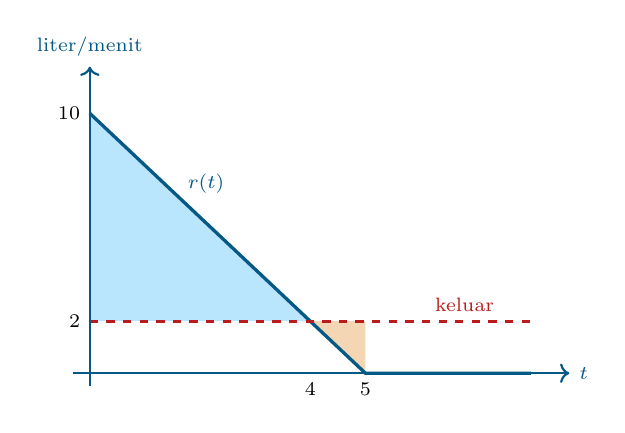
\begin{tikzpicture}[x=0.7cm,y=0.33cm]
\fill[skyl] (0,2)--(0,10)--(4,2)--cycle;
\fill[warmc!30] (4,2)--(5,0)--(5,2)--cycle;
\draw[very thick,mainc] (0,10)--(5,0)--(8,0);
\draw[very thick,brick,dashed] (0,2)--(8,2);
\draw[->,thick,mainc] (-0.3,0)--(8.7,0) node[right,font=\scriptsize]{$t$};
\draw[->,thick,mainc] (0,-0.5)--(0,11.8) node[above,font=\scriptsize]{liter/menit};
\foreach \t in {4,5}{\node[font=\scriptsize,below] at (\t,0) {$\t$};}
\node[font=\scriptsize,left] at (0,10) {$10$}; \node[font=\scriptsize,left] at (0,2) {$2$};
\node[font=\scriptsize,mainc,right] at (1.6,7.3) {$r(t)$};
\node[font=\scriptsize,brick,above] at (6.8,2) {keluar};
\end{tikzpicture}}}{\poin{8}}

\Needspace{24\baselineskip}
\tingkat{Tingkat Sulit}{soal 3 dan 4}
\soal{\gbr{Daerah $R$ dibatasi oleh kurva $y=\ln x$, garis $x=e$, dan sumbu $x$ (lihat gambar).\par\smallskip
(a) Hitung luas $R$ dengan integral parsial.\par
(b) Hitung volume benda putar jika $R$ diputar $360^\circ$ mengelilingi sumbu $x$.\par
(c) Nyatakan batas kiri $R$ sebagai $x=e^{y}$, lalu hitung luas $R$ dengan mengintegralkan terhadap $y$. Bandingkan dengan hasil (a).\par
(d) Hitung volume benda putar jika $R$ diputar $360^\circ$ mengelilingi sumbu $y$.}{%
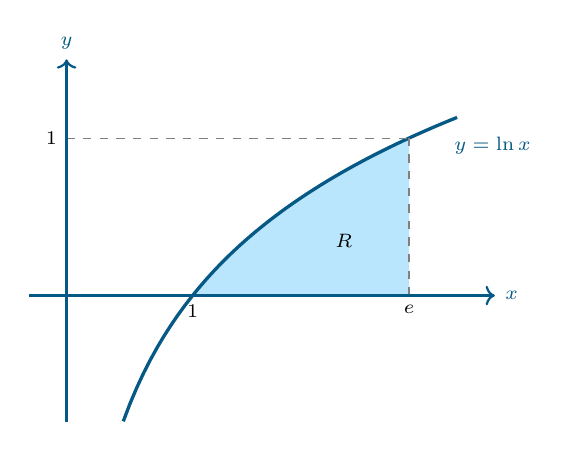
\begin{tikzpicture}[x=1.6cm,y=2.0cm]
\fill[skyl] (1,0)--(2.71828,0)--(2.71828,1)--plot[domain=2.71828:1,samples=40] ({\x},{ln(\x)})--cycle;
\draw[very thick,mainc,domain=0.45:3.1,samples=50] plot ({\x},{ln(\x)});
\draw[dashed,gray] (2.71828,0)--(2.71828,1) (0,1)--(2.71828,1);
\axs{-0.3}{-0.8}{3.4}{1.5}
\node[font=\scriptsize,below] at (1,0) {$1$};
\node[font=\scriptsize,below] at (2.71828,0) {$e$};
\node[font=\scriptsize,left] at (0,1) {$1$};
\node[font=\scriptsize,mainc,right] at (3.0,0.95) {$y=\ln x$};
\node[font=\scriptsize] at (2.2,0.35) {$R$};
\end{tikzpicture}}}{\poin{8}}
\soal{\gbr{Parabola $y=2x-x^2$ dan sumbu $x$ membatasi sebuah daerah (lihat gambar). Garis $y=mx$ dengan $0<m<2$ melalui titik asal dan memotong parabola di titik lain, sehingga daerah tersebut terbagi menjadi bagian atas (di atas garis) dan bagian bawah (di bawah garis).\par\smallskip
(a) Hitung luas seluruh daerah.\par
(b) Tentukan absis titik potong garis dan parabola selain titik asal, dinyatakan dalam $m$.\par
(c) Tunjukkan bahwa luas bagian atas adalah $\dfrac{(2-m)^3}{6}$.\par
(d) Tentukan $m$ agar garis membagi daerah menjadi dua bagian yang luasnya sama.}{%
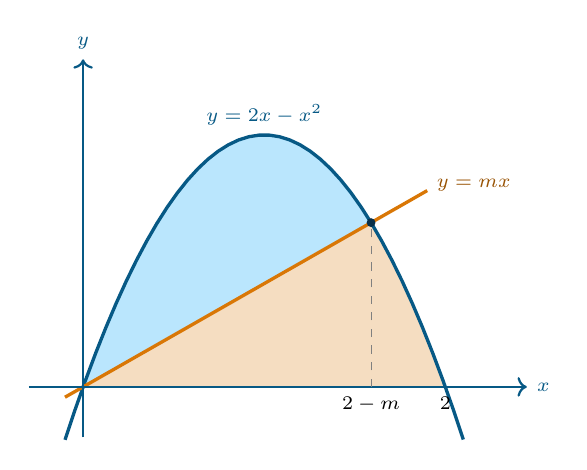
\begin{tikzpicture}[x=2.3cm,y=3.2cm]
\fill[skyl] (0,0)--(1.59,0.652)--plot[domain=1.59:0,samples=30] ({\x},{2*\x-\x*\x})--cycle;
\fill[warmc!25] (0,0)--(2,0)--plot[domain=2:1.59,samples=20] ({\x},{2*\x-\x*\x})--cycle;
\draw[very thick,mainc,domain=-0.1:2.1,samples=40] plot ({\x},{2*\x-\x*\x});
\draw[very thick,warmc] (-0.1,-0.041)--(1.9,0.779);
\axs{-0.3}{-0.2}{2.45}{1.3}
\fill[deepc] (1.59,0.652) circle (1.6pt);
\draw[dashed,gray] (1.59,0)--(1.59,0.652);
\node[font=\scriptsize,below] at (1.59,0) {$2-m$}; \node[font=\scriptsize,below] at (2,0) {$2$};
\node[font=\scriptsize,warmc!70!black,right] at (1.9,0.8) {$y=mx$};
\node[font=\scriptsize,mainc,above] at (1,1.0) {$y=2x-x^2$};
\end{tikzpicture}}}{\poin{8}}

\Needspace{26\baselineskip}
\tingkat{Tingkat HOTS}{soal 5}
\soal{\gbr{Sebuah vas bunga dibentuk dengan memutar daerah yang dibatasi kurva $x=\sqrt y$, sumbu $y$, dan garis $y=4$ mengelilingi sumbu $y$ (satuan panjang: dm; $1\ \text{dm}^3=1$ liter). Vas diisi air dari keran dengan debit tetap $2\pi$ liter/menit. Misalkan $h$ adalah kedalaman air (diukur dari dasar vas) dan $V(h)$ volume air pada kedalaman $h$.\par\smallskip
(a) Dengan membentuk integral, tunjukkan bahwa $V(h)=\dfrac{\pi h^2}{2}$.\par
(b) Berapa menit yang dibutuhkan hingga vas penuh?\par
(c) Pada kedalaman berapa vas terisi tepat setengah volumenya? Mengapa kedalaman itu lebih dari $2$ dm, padahal $2$ dm adalah setengah tinggi vas?\par
(d) Dengan Teorema Dasar Kalkulus, tentukan $\dfrac{dV}{dh}$, lalu hitung laju naiknya permukaan air $\dfrac{dh}{dt}$ saat $h=2$ dm.}{%
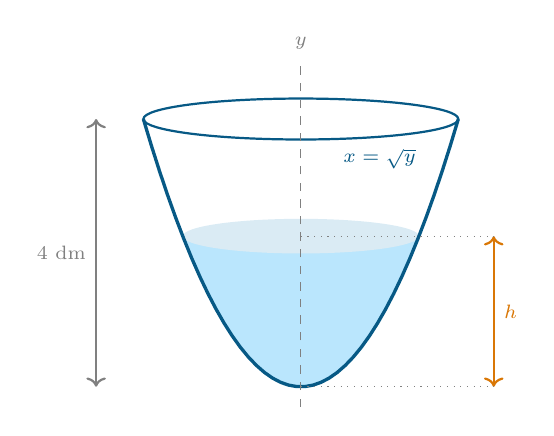
\begin{tikzpicture}[x=1.0cm,y=0.85cm]
\fill[skyl] (-1.5,2.25)--plot[domain=-1.5:1.5,samples=30] ({\x},{\x*\x})--(1.5,2.25)--cycle;
\fill[skyl!70!mainc!30] (0,2.25) ellipse (1.5cm and 0.22cm);
\draw[very thick,mainc,domain=-2:2,samples=40] plot ({\x},{\x*\x});
\draw[mainc,thick] (0,4) ellipse (2cm and 0.26cm);
\draw[dashed,gray] (0,-0.3)--(0,4.9) node[above,font=\scriptsize]{$y$};
\draw[<->,thick,warmc] (2.45,0)--(2.45,2.25) node[midway,right,font=\scriptsize]{$h$};
\draw[<->,thick,gray] (-2.6,0)--(-2.6,4) node[midway,left,font=\scriptsize]{$4$ dm};
\draw[dotted,gray] (0,2.25)--(2.45,2.25) (0,0)--(2.45,0);
\node[font=\scriptsize,mainc] at (1.0,3.4) {$x=\sqrt y$};
\end{tikzpicture}}}{\poin{8}}

% =====================================================================
\newpage
\bagian{Kunci Jawaban dan Pembahasan Singkat}{Untuk guru dan pembahasan mandiri}
\par\vspace{0.6em}{\bfseries\color{mainc}Kunci Pilihan Ganda}\par\vspace{0.3em}
\small
\begin{tabularx}{\linewidth}{@{}*{10}{>{\centering\arraybackslash}X}@{}}\hline \textbf{1} & \textbf{2} & \textbf{3} & \textbf{4} & \textbf{5} & \textbf{6} & \textbf{7} & \textbf{8} & \textbf{9} & \textbf{10}\\ \hline E & E & B & D & A & A & C & C & D & D\\ \hline\end{tabularx}\\[6pt]
\begin{tabularx}{\linewidth}{@{}*{10}{>{\centering\arraybackslash}X}@{}}\hline \textbf{11} & \textbf{12} & \textbf{13} & \textbf{14} & \textbf{15} & \textbf{16} & \textbf{17} & \textbf{18} & \textbf{19} & \textbf{20}\\ \hline B & B & D & C & E & C & E & B & A & A\\ \hline\end{tabularx}
\par\vspace{0.4em}{\bfseries\color{mainc}Kunci Isian Singkat:}\ \ 1) $2{,}5$\quad 2) $45$\quad 3) $\frac5{16}$\quad 4) $10$\quad 5) $\frac23$
\par\vspace{0.8em}{\bfseries\color{mainc}\normalsize Pembahasan Pilihan Ganda}\par\vspace{0.2em}
\small\begin{enumerate}[leftmargin=2em,itemsep=2pt,topsep=2pt]
\item[\textbf{1.}] \textbf{(E)} Teorema Dasar Kalkulus: $\int_1^3f=F(3)-F(1)$ tanpa perlu mencari $f$. $F(3)=27-18-2=7$ dan $F(1)=1-2-2=-3$, sehingga hasilnya $7-(-3)=10$. (Jebakan: $-10$ karena urutan dibalik, $7$ dan $-3$ hanya satu ujung, $4=7+(-3)$.)
\item[\textbf{2.}] \textbf{(E)} $\int\left(6x^{-1/2}+1\right)dx=12\sqrt x+x$. Nilainya $(24+4)-(12+1)=15$. (Jebakan: $12$ bila suku $1$ terlupa.)
\item[\textbf{3.}] \textbf{(B)} Pada $\int f(ax+b)\,dx$ kita membagi dengan $a$: $\int e^{2x}dx=\frac12e^{2x}$ dan $\int\cos4x\,dx=\frac14\sin4x$. (Jebakan: tidak membagi $a$, atau salah tanda.)
\item[\textbf{4.}] \textbf{(D)} Daerah di atas sumbu $x$ bernilai positif dan di bawahnya negatif: $\int_0^7f=6-4+5=7$. ($15$ adalah luas total, bukan integral; $-3$ muncul bila daerah ketiga dianggap negatif.)
\item[\textbf{5.}] \textbf{(A)} (i) $\int_{-1}^1x^2dx=\frac23$ dan $x^3$ fungsi ganjil bernilai $0$, jadi \textbf{B}. (ii) Yang benar $\ln|x|+C$; $\ln x$ hanya terdefinisi untuk $x>0$, jadi \textbf{S}. (iii) Teorema Dasar Kalkulus bagian pertama, \textbf{B}. Urutan: B, S, B.
\item[\textbf{6.}] \textbf{(A)} Misalkan $u=\ln x$, $du=\frac{dx}{x}$. Batas: $x=1\Rightarrow u=0$, $x=e\Rightarrow u=1$. Maka $\int_0^1u^2du=\frac13$. (Jebakan: $\frac{e^3-1}{3}$ bila batas tidak diubah.)
\item[\textbf{7.}] \textbf{(C)} Parsial dengan $u=\ln x$, $dv=x^2dx$: $\left[\frac{x^3}{3}\ln x\right]_1^e-\int_1^e\frac{x^2}{3}dx=\frac{e^3}{3}-\frac{e^3-1}{9}=\frac{2e^3+1}{9}$.
\item[\textbf{8.}] \textbf{(C)} Akar: $x=-2,0,2$. Di $[-2,0]$ kurva di atas sumbu dan di $[0,2]$ di bawah sumbu. Karena fungsi ganjil, kedua luas sama: $2\int_0^2(4x-x^3)dx=2\left[2x^2-\frac{x^4}{4}\right]_0^2=2\cdot4=8$. (Jebakan: $\int_{-2}^2=0$.)
\item[\textbf{9.}] \textbf{(D)} $V=\pi\int_0^\pi\sin^2x\,dx=\pi\int_0^\pi\frac{1-\cos2x}{2}dx=\pi\cdot\frac\pi2=\frac{\pi^2}{2}$. (Jebakan: $2\pi$ bila lupa mengkuadratkan; $\pi^2$ bila lupa $\frac12$.)
\item[\textbf{10.}] \textbf{(D)} $v=\int(6-2t)dt=6t-t^2+C$ dan $v(0)=-5$, sehingga $v=-(t-1)(t-5)$. Drone mundur pada $0\le t<1$ dan maju pada $1<t\le5$. Dengan $G(t)=-\frac{t^3}{3}+3t^2-5t$: $G(1)=-\frac73$, $G(5)=\frac{25}{3}$. Jarak $=\left|G(1)-G(0)\right|+\left|G(5)-G(1)\right|=\frac73+\frac{32}{3}=13$. (Perpindahan hanya $\frac{25}{3}$.)
\item[\textbf{11.}] \textbf{(B)} $f'(x)=3x^2-4x+c$ dan $f'(1)=0\Rightarrow c=1$. Lalu $f(x)=x^3-2x^2+x+k$ dan $f(0)=3\Rightarrow k=3$. Jadi $f(2)=8-8+2+3=5$. (Jebakan: lupa konstanta $c$ menghasilkan $3$.)
\item[\textbf{12.}] \textbf{(B)} $\sin^3x\cos^2x=(1-\cos^2x)\cos^2x\sin x$. Misalkan $u=\cos x$, $du=-\sin x\,dx$, batas $x:0\to\frac\pi2$ menjadi $u:1\to0$: $\int_0^1(u^2-u^4)du=\frac13-\frac15=\frac2{15}$.
\item[\textbf{13.}] \textbf{(D)} Di $[1,2]$ kurva $\frac8x$ berada di atas $x^2$ (sama di $x=2$). $L=\int_1^2\left(\frac8x-x^2\right)dx=\left[8\ln x-\frac{x^3}{3}\right]_1^2=8\ln2-\frac83+\frac13=8\ln2-\frac73$.
\item[\textbf{14.}] \textbf{(C)} Misalkan $u=x+1$, maka $x=u-1$ dan batas menjadi $1$ sampai $4$: $\int_1^4\frac{u-1}{\sqrt u}du=\left[\frac23u^{3/2}-2u^{1/2}\right]_1^4=\left(\frac{16}{3}-4\right)-\left(\frac23-2\right)=\frac83$.
\item[\textbf{15.}] \textbf{(E)} (1) Dengan $u=x^2+1$, $x\,dx=\frac12du$, batas $1\to5$: $\frac12\cdot12=6$, \textbf{benar}. (2) Dengan $u=2x+1$, $dx=\frac12du$, batas $1\to5$: $\frac12\cdot12=6\neq12$, \textbf{salah}. (3) $12+2\cdot4=20$, \textbf{benar}. (4) Dengan $u=6-x$ batas $x:1\to5$ menjadi $u:5\to1$ dan $dx=-du$, sehingga hasilnya $+12$, bukan $-12$: \textbf{salah}. Yang benar: (1) dan (3).
\item[\textbf{16.}] \textbf{(C)} Misalkan $I=\int e^x\sin x\,dx$. Parsial dua kali menghasilkan $I=e^x\sin x-e^x\cos x-I$, sehingga $I=\frac{e^x(\sin x-\cos x)}{2}$. Maka $\int_0^\pi=\frac{e^\pi(0+1)-(0-1)}{2}=\frac{e^\pi+1}{2}$.
\item[\textbf{17.}] \textbf{(E)} Titik potong $x=\pm1$ dan $2-x^2\ge x^2$ di antaranya. Metode cincin: $V=\pi\int_{-1}^1\left[(2-x^2)^2-x^4\right]dx=\pi\int_{-1}^1(4-4x^2)dx=\pi\left[4x-\frac{4x^3}{3}\right]_{-1}^1=\frac{16\pi}{3}$. (Jebakan: $\frac{64\pi}{15}$ bila selisihnya yang dikuadratkan.)
\item[\textbf{18.}] \textbf{(B)} Lebar tiap persegi panjang $\Delta x=\frac2n$ dan $x_k=1+\frac{2k}{n}$, sehingga limit jumlah sama dengan $\int_1^3x^2dx=\frac{27-1}{3}=\frac{26}{3}$. (Jebakan: $\frac83$ bila selang dibaca $[0,2]$.)
\item[\textbf{19.}] \textbf{(A)} $f'(x)=2ax+b$. Pernyataan (1): $f'(1)=0\Rightarrow b=-2a$, sehingga $\int_0^3(ax^2-2ax)dx=a\left[\frac{x^3}{3}-x^2\right]_0^3=a(9-9)=0$ untuk semua $a$. Jadi (1) saja cukup. Pernyataan (2): $a+b=-1$ dan $\int_0^3f=9a+\frac92b=\frac92(a-1)$, bergantung pada $a$ yang belum diketahui, jadi (2) saja tidak cukup.
\item[\textbf{20.}] \textbf{(A)} Dengan luas bertanda: $F(1)=1$, $F(3)=5$, $F(4)=6$, $F(5)=5$, $F(6)=3$, $F(7)=2$, $F(8)=3$. (1) $F'=f>0$ pada $(0,4)$ dan $f<0$ pada $(4,7)$, maksimum $F(4)=6$: \textbf{benar}. (2) $F(6)=3$: \textbf{benar}. (3) Pada $3<x<4$ nilai $f>0$ sehingga $F$ masih naik: \textbf{salah}. (4) $\int_0^8f=F(8)=3$; angka $11=7+4$ adalah luas total, bukan integral: \textbf{salah}.
\end{enumerate}
\par\Needspace{6\baselineskip}\vspace{0.6em}{\bfseries\color{mainc}\normalsize Pembahasan Isian Singkat}\par\vspace{0.2em}
\small\begin{enumerate}[leftmargin=2em,itemsep=2pt,topsep=2pt]
\item[\textbf{1.}] \textbf{Jawaban: $2{,}5$.} $\left[2x^2-3x\right]_1^a=2a^2-3a+1=6\Rightarrow2a^2-3a-5=0\Rightarrow(2a-5)(a+1)=0$. Karena $a>1$, $a=\frac52=2{,}5$.
\item[\textbf{2.}] \textbf{Jawaban: $45$.} Air yang masuk sama dengan luas di bawah grafik: trapesium $\frac{2+6}{2}\cdot4=16$, persegi panjang $6\cdot2=12$, segitiga $\frac12\cdot4\cdot6=12$; total $40$ liter. Ditambah $5$ liter awal: $45$ liter.
\item[\textbf{3.}] \textbf{Jawaban: $\frac5{16}$.} $\sin3x\cos x=\frac12(\sin4x+\sin2x)$. Maka $\frac12\left[-\frac{\cos4x}{4}-\frac{\cos2x}{2}\right]_0^{\pi/6}=\frac12\left[\left(\frac18-\frac14\right)-\left(-\frac14-\frac12\right)\right]=\frac12\cdot\frac58=\frac5{16}$.
\item[\textbf{4.}] \textbf{Jawaban: $10$.} Integral $\int_0^1f(t)\,dt$ adalah sebuah bilangan; misalkan $c$. Maka $f(x)=3x^2+2c$ dan $c=\int_0^1(3x^2+2c)dx=1+2c$, sehingga $c=-1$. Jadi $f(x)=3x^2-2$ dan $f(2)=10$.
\item[\textbf{5.}] \textbf{Jawaban: $\frac23$.} Gradien di $x=2$ adalah $2x=4$, sehingga $g:y=4x-4$ memotong sumbu $x$ di $x=1$. Luas $=\int_0^2x^2dx-\int_1^2(4x-4)dx=\frac83-2=\frac23$ (luas di bawah parabola dikurangi segitiga di bawah garis $g$).
\end{enumerate}
\par\Needspace{8\baselineskip}\vspace{0.6em}{\bfseries\color{mainc}\normalsize Pembahasan dan Pedoman Penskoran Uraian}\par\vspace{0.2em}
\small\begin{enumerate}[leftmargin=2em,itemsep=3pt,topsep=2pt]
\item[\textbf{1.}] (a) $4x-x^2=x\Rightarrow x(3-x)=0$, jadi $(0,0)$ dan $(3,3)$. (b) $L=\int_0^3(3x-x^2)dx=\left[\frac{3x^2}{2}-\frac{x^3}{3}\right]_0^3=\frac{27}{2}-9=\frac92$. (c) Cincin: $V=\pi\int_0^3\left[(4x-x^2)^2-x^2\right]dx=\pi\int_0^3(15x^2-8x^3+x^4)dx=\pi\left[5x^3-2x^4+\frac{x^5}{5}\right]_0^3=\pi\left(135-162+\frac{243}{5}\right)=\frac{108\pi}{5}$. (d) Selisih kurva $g(x)=3x-x^2=x(3-x)$ memenuhi $g(3-x)=g(x)$, jadi simetris terhadap $x=\frac32$; garis $x=\frac32$ membagi $D$ dua sama besar. Cek: $\int_0^{3/2}(3x-x^2)dx=\frac{27}{8}-\frac98=\frac94=\frac12L$. Jadi $k=\frac32$. \\ \textit{Penskoran: (a) 1 poin; (b) 2 poin; (c) 3 poin; (d) 2 poin.}
\item[\textbf{2.}] (a) $V'(t)=r(t)-2=8-2t$. $V'=0$ pada $t=4$, dan $V'$ berganti dari positif ke negatif, jadi volume maksimum pada $t=4$. (b) $V(t)=10+\int_0^t(8-2s)ds=10+8t-t^2$. $V(4)=10+32-16=26$ liter. (c) Air masuk $\int_0^5(10-2t)dt=25$ liter; air keluar $2\cdot5=10$ liter; $V(5)=10+25-10=25$ liter. Cocok dengan $V(5)=10+40-25=25$. (d) Mulai $t=5$ tidak ada air masuk, sehingga volume berkurang $2$ liter/menit dari $25$ liter: butuh $\frac{25}{2}=12{,}5$ menit. Bak kosong pada menit ke-$17{,}5$. \\ \textit{Penskoran: (a) 2 poin; (b) 2 poin; (c) 2 poin; (d) 2 poin.}
\item[\textbf{3.}] (a) $\int_1^e\ln x\,dx$ dengan $u=\ln x$, $dv=dx$: $\left[x\ln x-x\right]_1^e=(e-e)-(0-1)=1$. (b) $V=\pi\int_1^e(\ln x)^2dx$. Parsial dua kali: $\int(\ln x)^2dx=x(\ln x)^2-2x\ln x+2x$. Maka $V=\pi\left[(e-2e+2e)-(0-0+2)\right]=\pi(e-2)$. (c) Dari $y=\ln x$ diperoleh $x=e^y$, $0\le y\le1$; batas kanan $x=e$. $L=\int_0^1(e-e^y)dy=\left[ey-e^y\right]_0^1=(e-e)-(0-1)=1$. Sama dengan (a). (d) Cincin dengan jari-jari luar $e$ dan dalam $e^y$: $V=\pi\int_0^1\left(e^2-e^{2y}\right)dy=\pi\left[e^2y-\frac{e^{2y}}{2}\right]_0^1=\pi\left(e^2-\frac{e^2}{2}+\frac12\right)=\frac{\pi(e^2+1)}{2}$. \\ \textit{Penskoran: (a) 2 poin; (b) 3 poin; (c) 1 poin; (d) 2 poin.}
\item[\textbf{4.}] (a) $\int_0^2(2x-x^2)dx=\left[x^2-\frac{x^3}{3}\right]_0^2=4-\frac83=\frac43$. (b) $2x-x^2=mx\Rightarrow x(2-m-x)=0$, jadi $x=2-m$. (c) Bagian atas $=\int_0^{2-m}\left[(2x-x^2)-mx\right]dx=\int_0^{2-m}\left[(2-m)x-x^2\right]dx=(2-m)\frac{(2-m)^2}{2}-\frac{(2-m)^3}{3}=\frac{(2-m)^3}{6}$. (d) Syarat $\frac{(2-m)^3}{6}=\frac12\cdot\frac43=\frac23$, sehingga $(2-m)^3=4$ dan $m=2-\sqrt[3]4\approx0{,}41$ (memenuhi $0<m<2$). \\ \textit{Penskoran: (a) 1 poin; (b) 2 poin; (c) 3 poin; (d) 2 poin.}
\item[\textbf{5.}] (a) Pada kedalaman $y$, irisan datar berupa cakram berjari-jari $x=\sqrt y$ sehingga luasnya $\pi y$. $V(h)=\pi\int_0^h\left(\sqrt y\right)^2dy=\pi\int_0^hy\,dy=\frac{\pi h^2}{2}$. (b) Vas penuh pada $h=4$: $V(4)=8\pi$ liter. Waktu $=\frac{8\pi}{2\pi}=4$ menit. (c) Setengah volume $=4\pi$: $\frac{\pi h^2}{2}=4\pi\Rightarrow h^2=8\Rightarrow h=2\sqrt2\approx2{,}83$ dm. Vas melebar ke atas: bagian bawah sempit dan menampung sedikit air, sedangkan bagian atas menampung banyak. Karena itu separuh volume baru tercapai setelah permukaan melewati setengah tinggi ($V(2)=2\pi$ baru seperempat dari $8\pi$). (d) $\frac{dV}{dh}=\frac{d}{dh}\left[\pi\int_0^hy\,dy\right]=\pi h$, yaitu luas permukaan air. Dari $\frac{dV}{dt}=\frac{dV}{dh}\cdot\frac{dh}{dt}$ dengan $\frac{dV}{dt}=2\pi$: $\frac{dh}{dt}=\frac{2\pi}{\pi h}=\frac2h$. Saat $h=2$: $\frac{dh}{dt}=1$ dm/menit. \\ \textit{Penskoran: (a) 2 poin; (b) 1 poin; (c) 2 poin; (d) 3 poin.}
\end{enumerate}
\end{document}
